
\section{Reinterpretation with Prompt Analyses}\label{sec:ch5-recastingPrompt}

% Depending on the lifetime, a part of the LLP decays will always happen
% outside the detector, leading to a \MET signature if the LLP is
% electrically and color neutral. Likewise, some part of the LLP decays will always appear
% ``promptly". Prompt searches with and without \MET can therefore provide
% additional, corroborating constraints on models with LLPs. Therefore, it is
% important to understand the sensitivity of prompt searches to displaced objects.

% Reinterpreting prompt searches in the context of LLPs is, however,
% quite nontrivial, because not all prompt searches make explicit
% requirements on the primary vertex. Moreover, it is not documented how
% reconstruction efficiencies drop as a function of small displacement.
% Thus, the reinterpretation of prompt searches in the context of LLPs is
% currently best done within the collaborations themselves.

Since the decay time probability of an unstable particle follows an
exponential decay law (dependent upon the mean lifetime), some percentage of the decays of the LLP
will occure outside the detector, leading to an \MET signature if the LLP is
electrically and color neutral. Likewise, some part of the LLP decays
can appear ``promptly". Prompt searches with and without \MET can
therefore provide additional, corroborating constraints on models with
LLPs, especially for short lifetimes. Therefore, it is important to
understand the sensitivity of prompt searches to displaced objects.

Reinterpreting prompt searches in the context of LLPs is, however,
quite nontrivial, because {\it a)} prompt searches may or may not make
explicit requirements on the primary vertex and {\it b)} it is
currently not documented how reconstruction efficiencies drop as a
function of small displacement. Thus, the reinterpretation of prompt
searches in the context of LLPs is currently best done within the
collaborations themselves.

An example of such an experiment-internal reinterpretation can be found in a CMS
search for an RPV SUSY model where pair-production of stops each proceed through
an R-parity violating decay to a $b$ quark and a lepton. A dedicated long-lived
search for this model exists in the $e\mu$ channel~\cite{CMS-PAS-EXO-16-022}.
This search includes selection criteria which require the transverse impact
parameter to the interaction point be greater than 10~$\mu$m. This maximizes
sensitivity to the long-lived model and greatly reduces standard model
backgrounds. It also necessarily highly reduces the sensitivity of the search at
low stop lifetime. The exclusion curve in the stop lifetime ($c\tau$) vs. top
squark mass is shown in the left frame of Figure~\ref{fig:exo-16}.

A reinterpretation was performed of a search for pair-production of second
generation leptoquarks (LQs)~\cite{CMS-PAS-EXO-16-007,Sirunyan:2018ryt}. In this model, massive
leptoquarks are pair-produced. Each of these bosons then decays to a muon and
$c$ quark, leading to a final state with two muons and two jets from $c$ quarks.
In the prompt limit of the RPV SUSY model with a final state of two muons and
two jets from $b$ quarks, the kinematics of the LQs are nearly identical. In the
LQ search, no selection is made on jet flavor. The LQ search uses final
selections which are optimized to the event kinematics for each LQ mass
hypothesis, but the search in general strives to remain as model-independent as
possible. In this case, the reinterpretation was simply performed using the
original LQ analysis, and replacing the signal samples with the long-lived RPV
samples, only taking into account the reduced branching fraction to the final state with two
muons and two jets. The expected and observed exclusion curves of the
reinterpretation are shown in the right frame of Figure~\ref{fig:exo-16}.

The reinterpretation gives large improvements for lifetimes $\leq1$mm, and as
expected, contributes little in the large lifetime limit. This type of
reinterpretation is valuable not only because it extends coverage of a given
model, but also because it helps guide the analysts performing the dedicated
search to focus their efforts in areas which are truly uncovered.

Reinterpretations like this one, which provide meaningful results without
placing a large burden on analysis teams, should be highly encouraged. Other reinterpretations along
these lines can be found in Refs.~\cite{ATLAS-CONF-2014-037,Sirunyan:2018vjp,Aaboud:2018iil}. Another relatively simple
reinterpretation is Ref.~\cite{ATLAS-CONF-2018-003}, although in this case, it
should be noted that the original analysis was modified in a simple way, that is,
the reliance on tracking information to identify jets and suppress non-collision background was
removed, in order to be sensitive to long-lived gluinos.

\begin{figure}[t]
\begin{center}
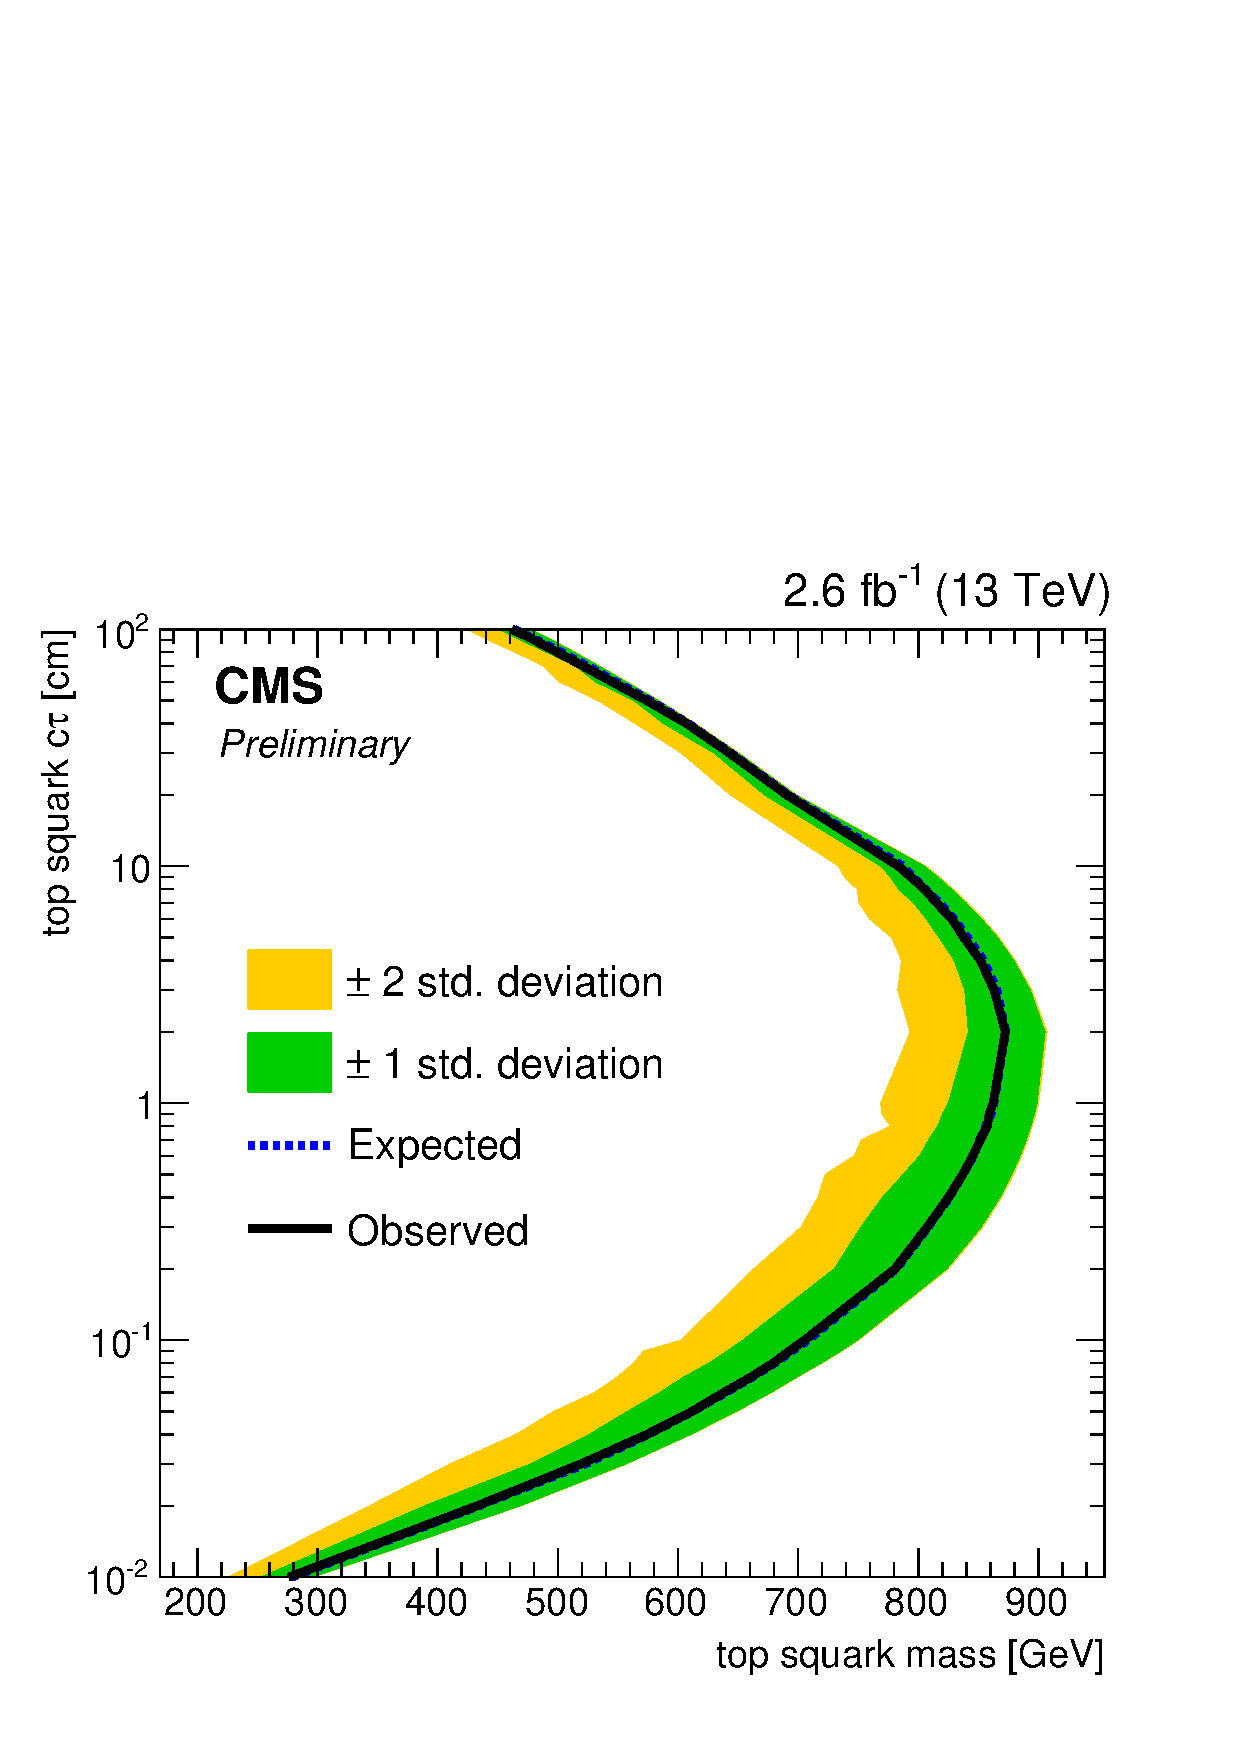
\includegraphics[width=0.45\textwidth,angle=0]{ch5-figures/CMS-PAS-EXO-16-022_Figure_004.pdf}
% 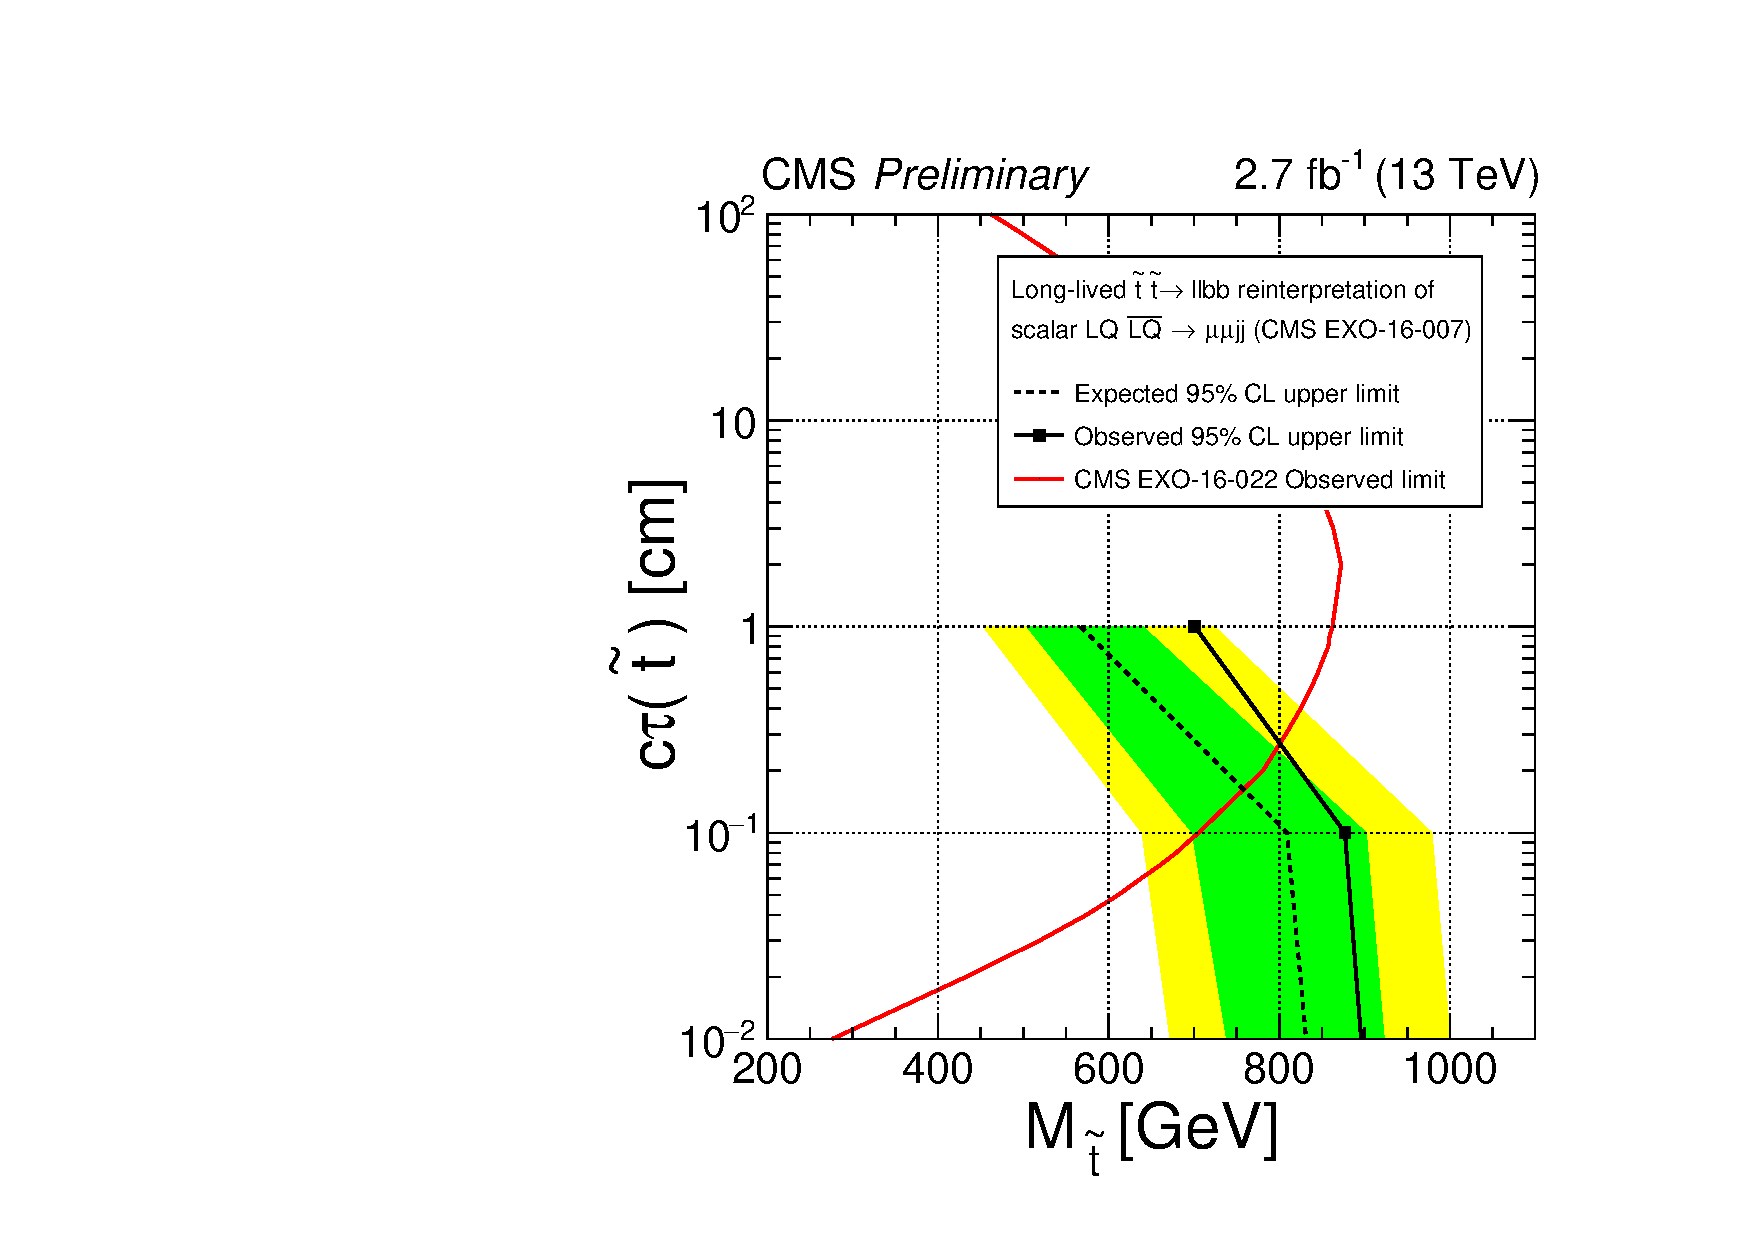
\includegraphics[width=0.5\textwidth,angle=0]{ch5-figures/CMS-PAS-EXO-16-007_Figure-aux_001.pdf}
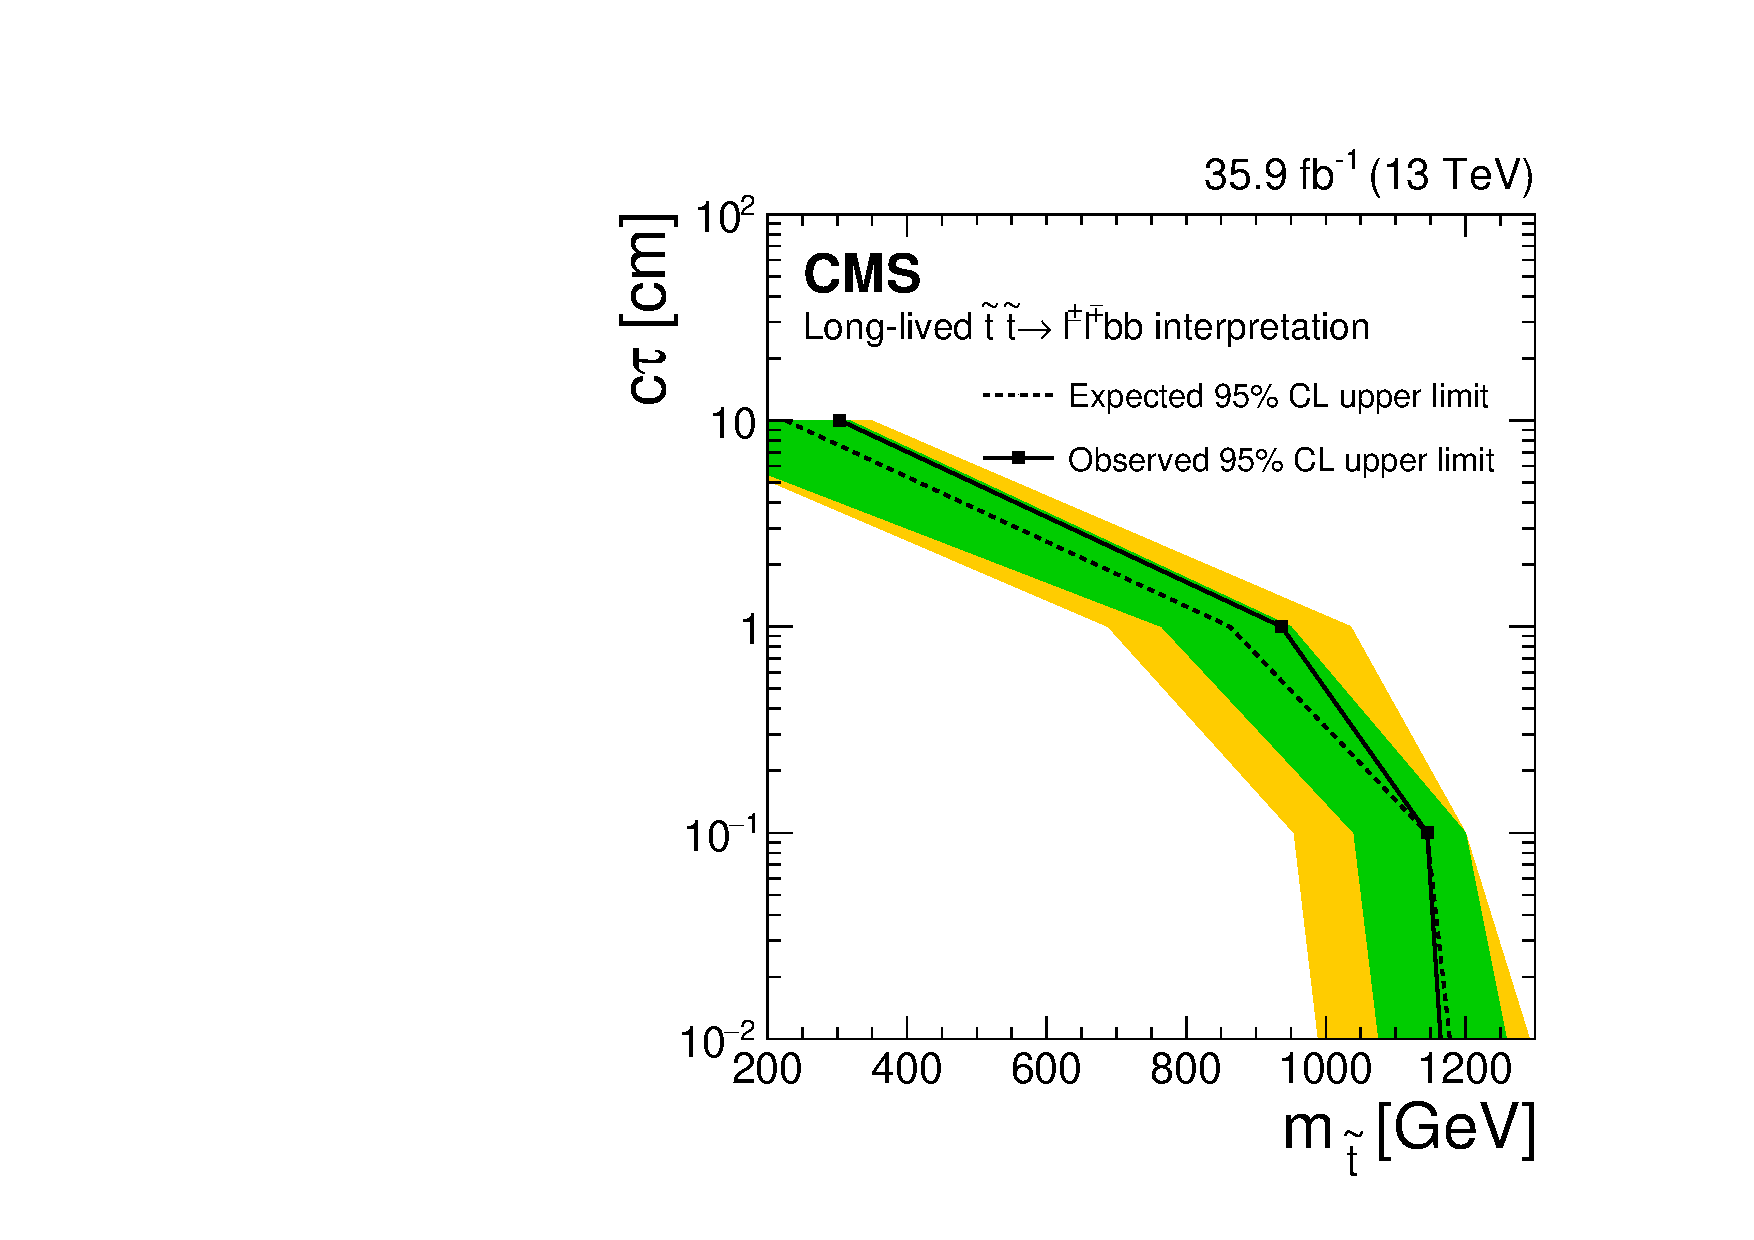
\includegraphics[width=0.45\textwidth,angle=0]{ch5-figures/CMS-EXO-17-003_Figure_010.pdf}
\end{center}
\caption{{\bf Left:} Expected and observed $95\%$ confidence level limits in the $c\tau$-M$_{\tilde{t}}$ plane from the displaced lepton search~\cite{CMS-PAS-EXO-16-022} for pair-production of long-lived stops decaying to $b$ quarks and leptons. {\bf Right:} Exclusion on the pair-production of long-lived stops decaying to $b$ quarks and leptons in the $c\tau$-M$_{\tilde{t}}$ plane, from the prompt reinterpretation of the second generation LQ search~\cite{Sirunyan:2018ryt}.} %Exclusion in the $c\tau$-M$_{\tilde{t}}$ plane from the prompt reinterpretation of pair-production of long-lived stops decaying to $b$ quarks and leptons~\cite{Sirunyan:2018ryt}. }%Exclusion from the dedicated long-lived search in Ref.~\cite{CMS-PAS-EXO-16-022} is overlaid with a solid red line~\cite{CMS-EXO-16-007url}.}
\label{fig:exo-16}
\end{figure}




